In this section we are going to show some mockups of the system regarding mobile application only. On the RASD document we have presented some web application mockups and how they can be derived from mobile ones; for this reason we suppose UI developers will be able to retrieve correct web application mockups from the followers.\\
During the design of mockups we have followed exactly what is presented on UX diagrams; for obvious reasons we can't show all the screens that are on the UX diagrams, however lot of them has been created trying to clarify precisely how the user should interact with the system.\\
The mockups we are going to present are the following:
\begin{itemize}
	\item \textbf{Homepage}: This mockup shows the external homepage of the system. This can be seen by anyone who downloads the application and want to register or login.
	\item \textbf{Calendar Page}: In this mockup we show main page of the system where users are able to seen their meetings and travels. We offer the possibility to easily switch between daily, weekly and monthly views and create a new meeting. Moreover we show the meeting and travel details page where users can see more deeply their events.
	\item \textbf{Notifications}: We have designed a notification page where a warning and an invitation are pending. User can click on warning to open the overlapping meetings page where it can accept, decline or reschedule each of them; a rescheduling proposal page has been designed too. In addition, the user can choose to see in details the meeting who has been invited to.
	\item \textbf{Settings}: In this mockup can be easily seen the current status, the current default location and daily breaks. We have showed how the user can edit its preference list, marking as inactive travel means that it doesn't want to use. Moreover we have created mockups related to the process of adding a new constraint. The system suggests the user every time all the possibilities that it can choose in creating the new constraint.
\end{itemize}

\begin{figure}[h]
	\centering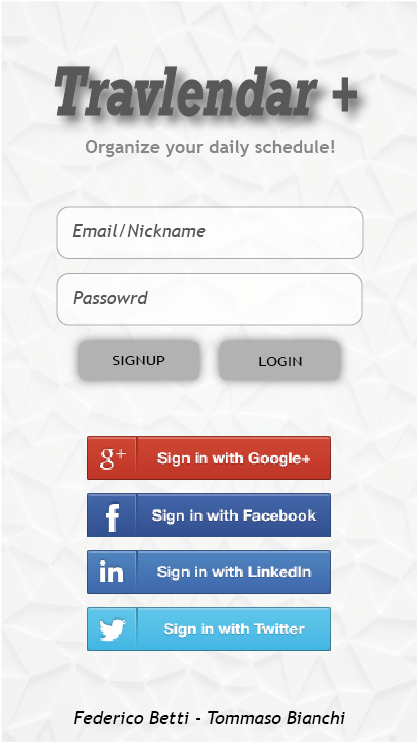
\includegraphics[scale = 0.35]{Images/Mockups/HomePage.png}{}
	\caption{External Homepage}
\end{figure}

\begin{figure}[h]
\centering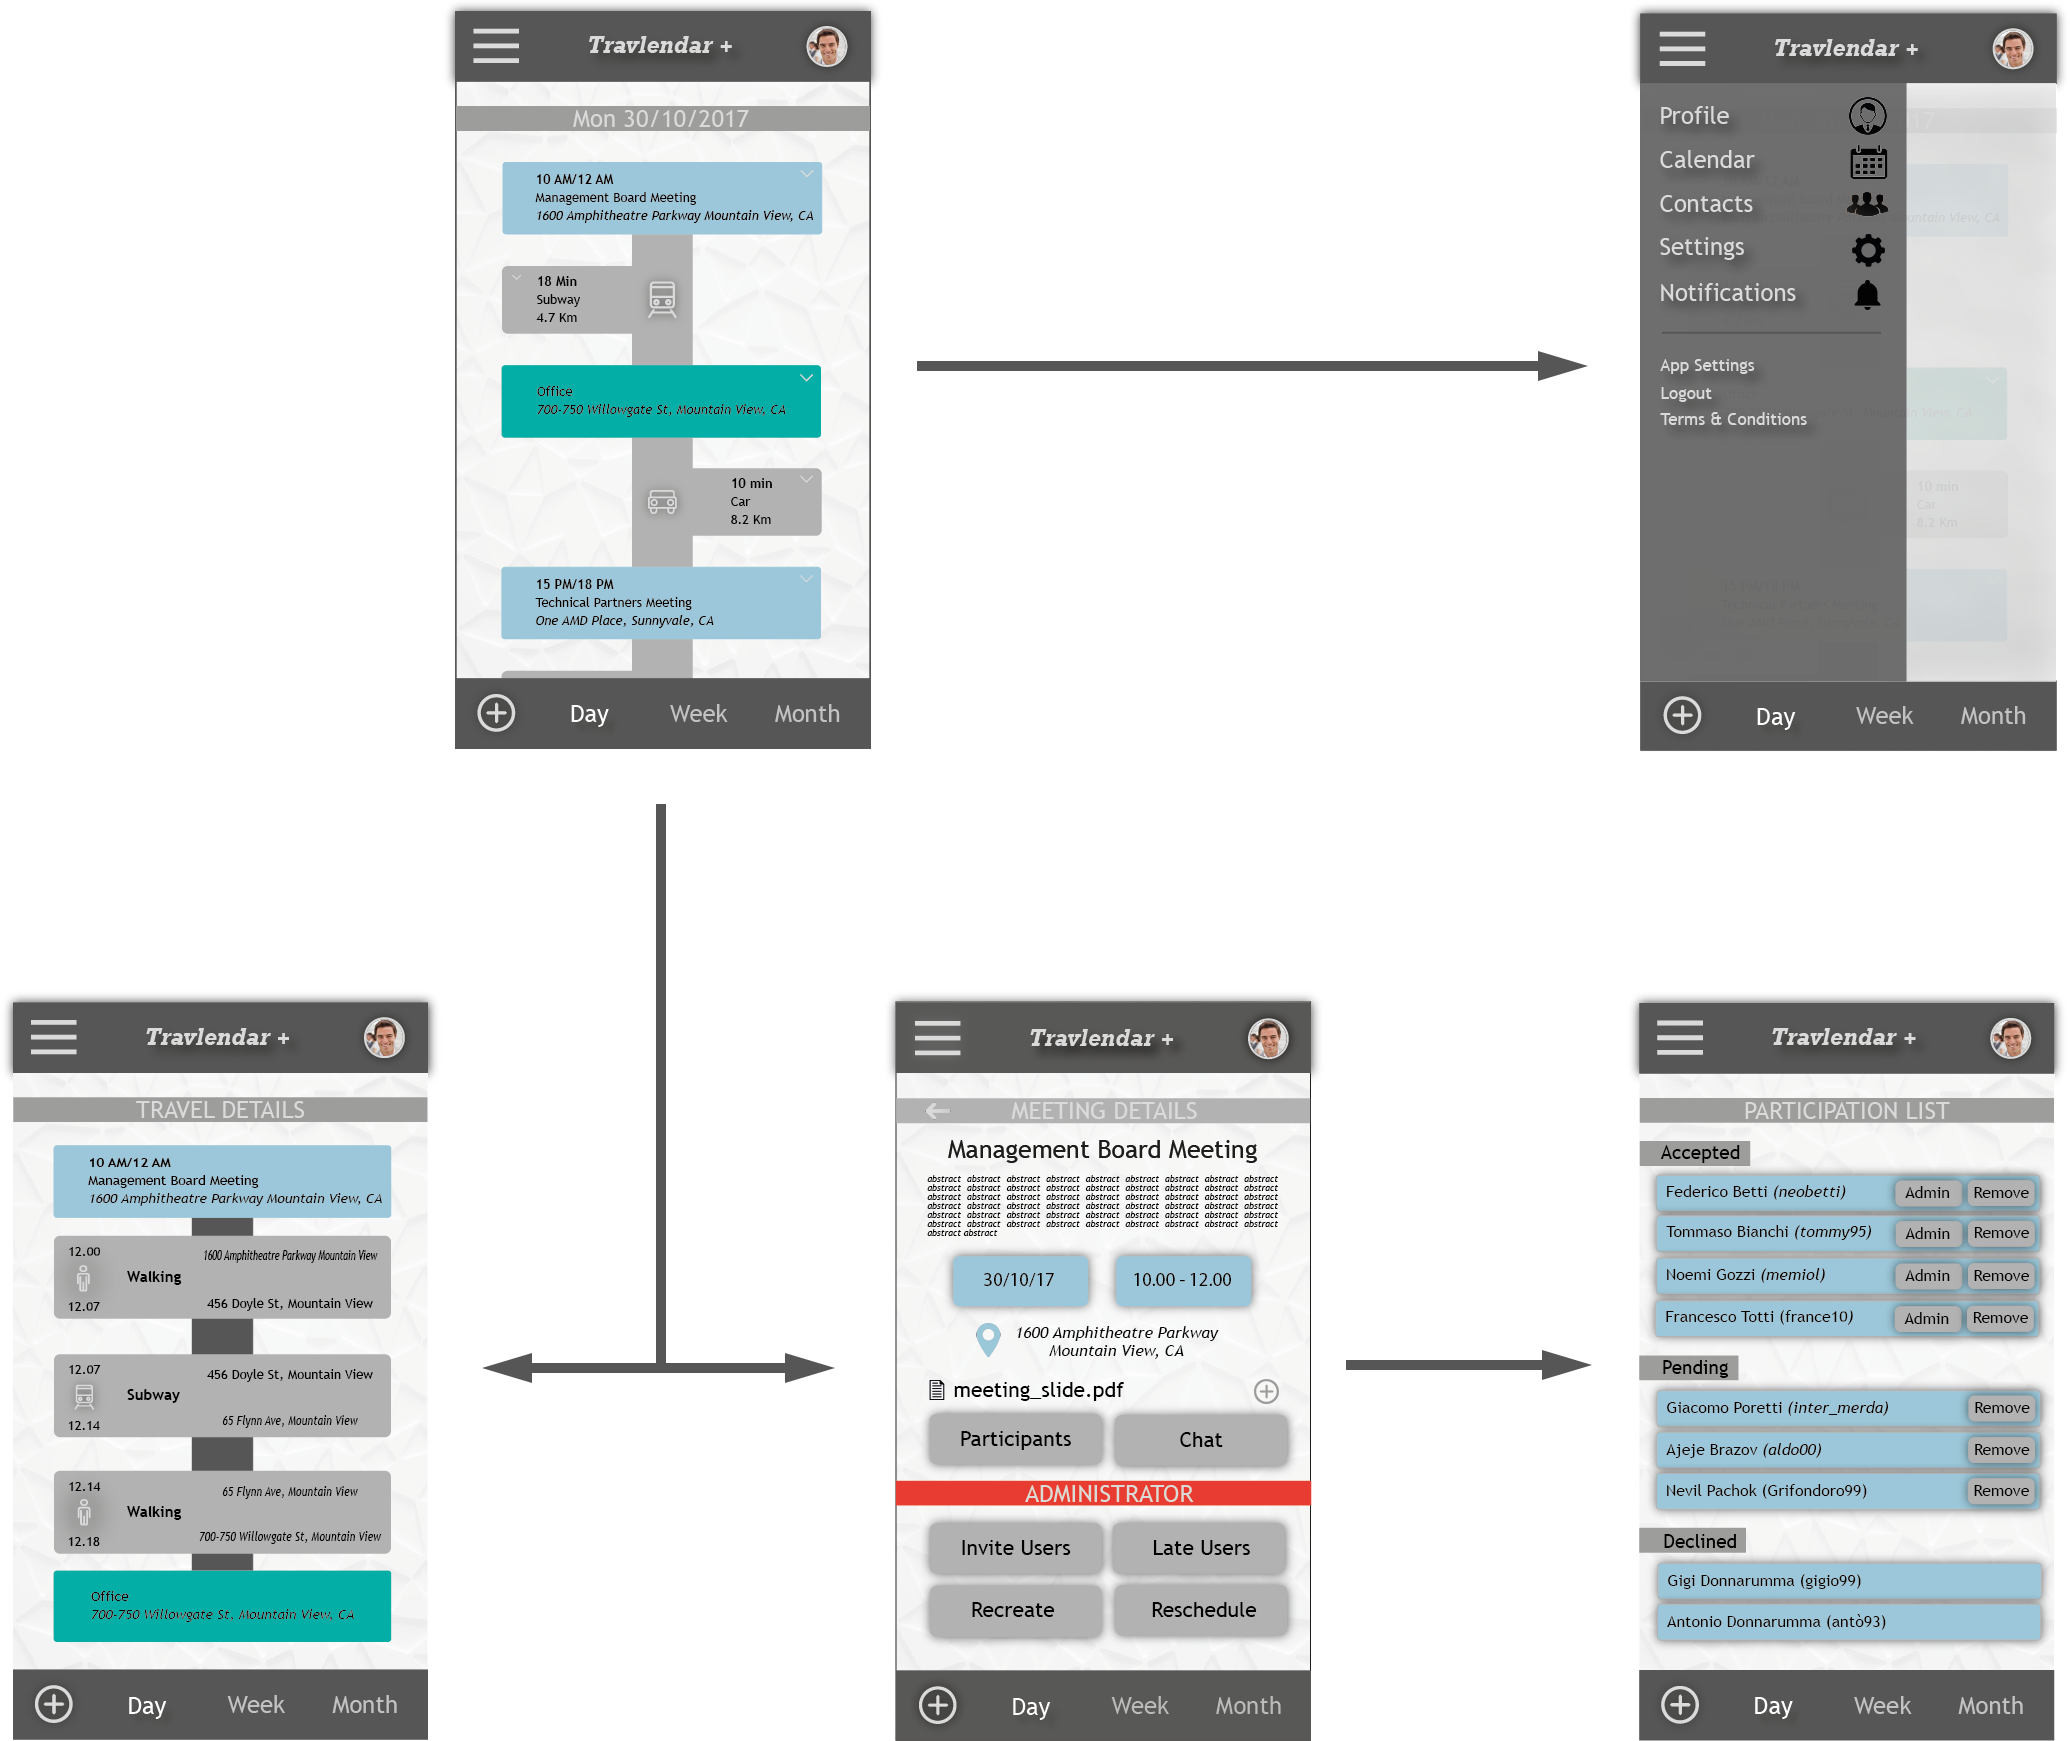
\includegraphics[width = \textwidth, scale = 0.3]{Images/Mockups/CalendarPage+.png}{}
\caption{Calendar Page Mockup}
\end{figure}

\begin{figure}[h]
\centering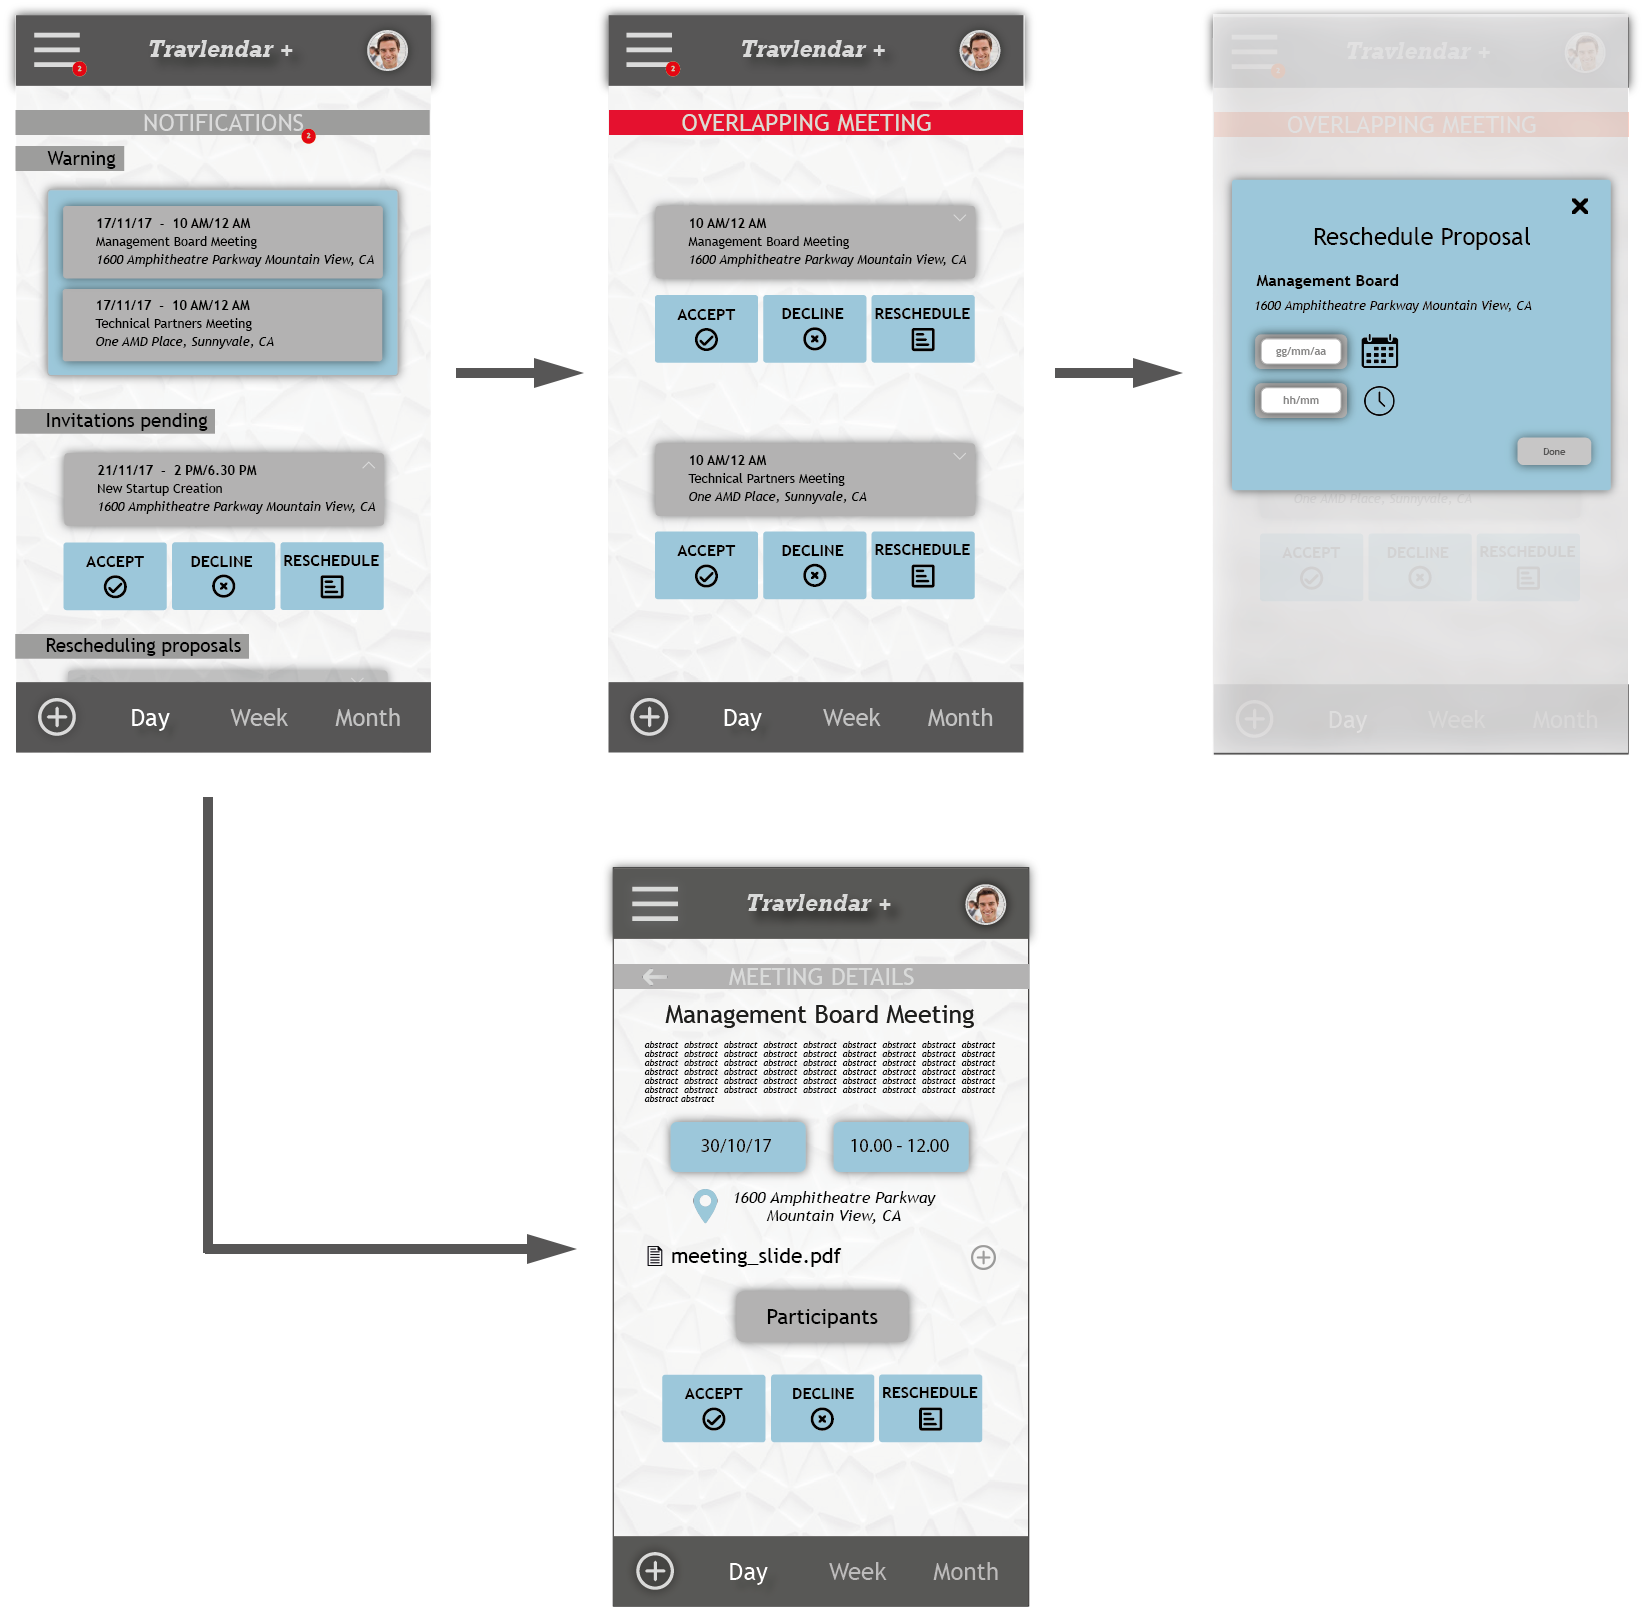
\includegraphics[scale = 0.3]{Images/Mockups/Notifications+.png}{}
\caption{Notifications Mockup}
\end{figure}

\begin{figure}[h]
\centering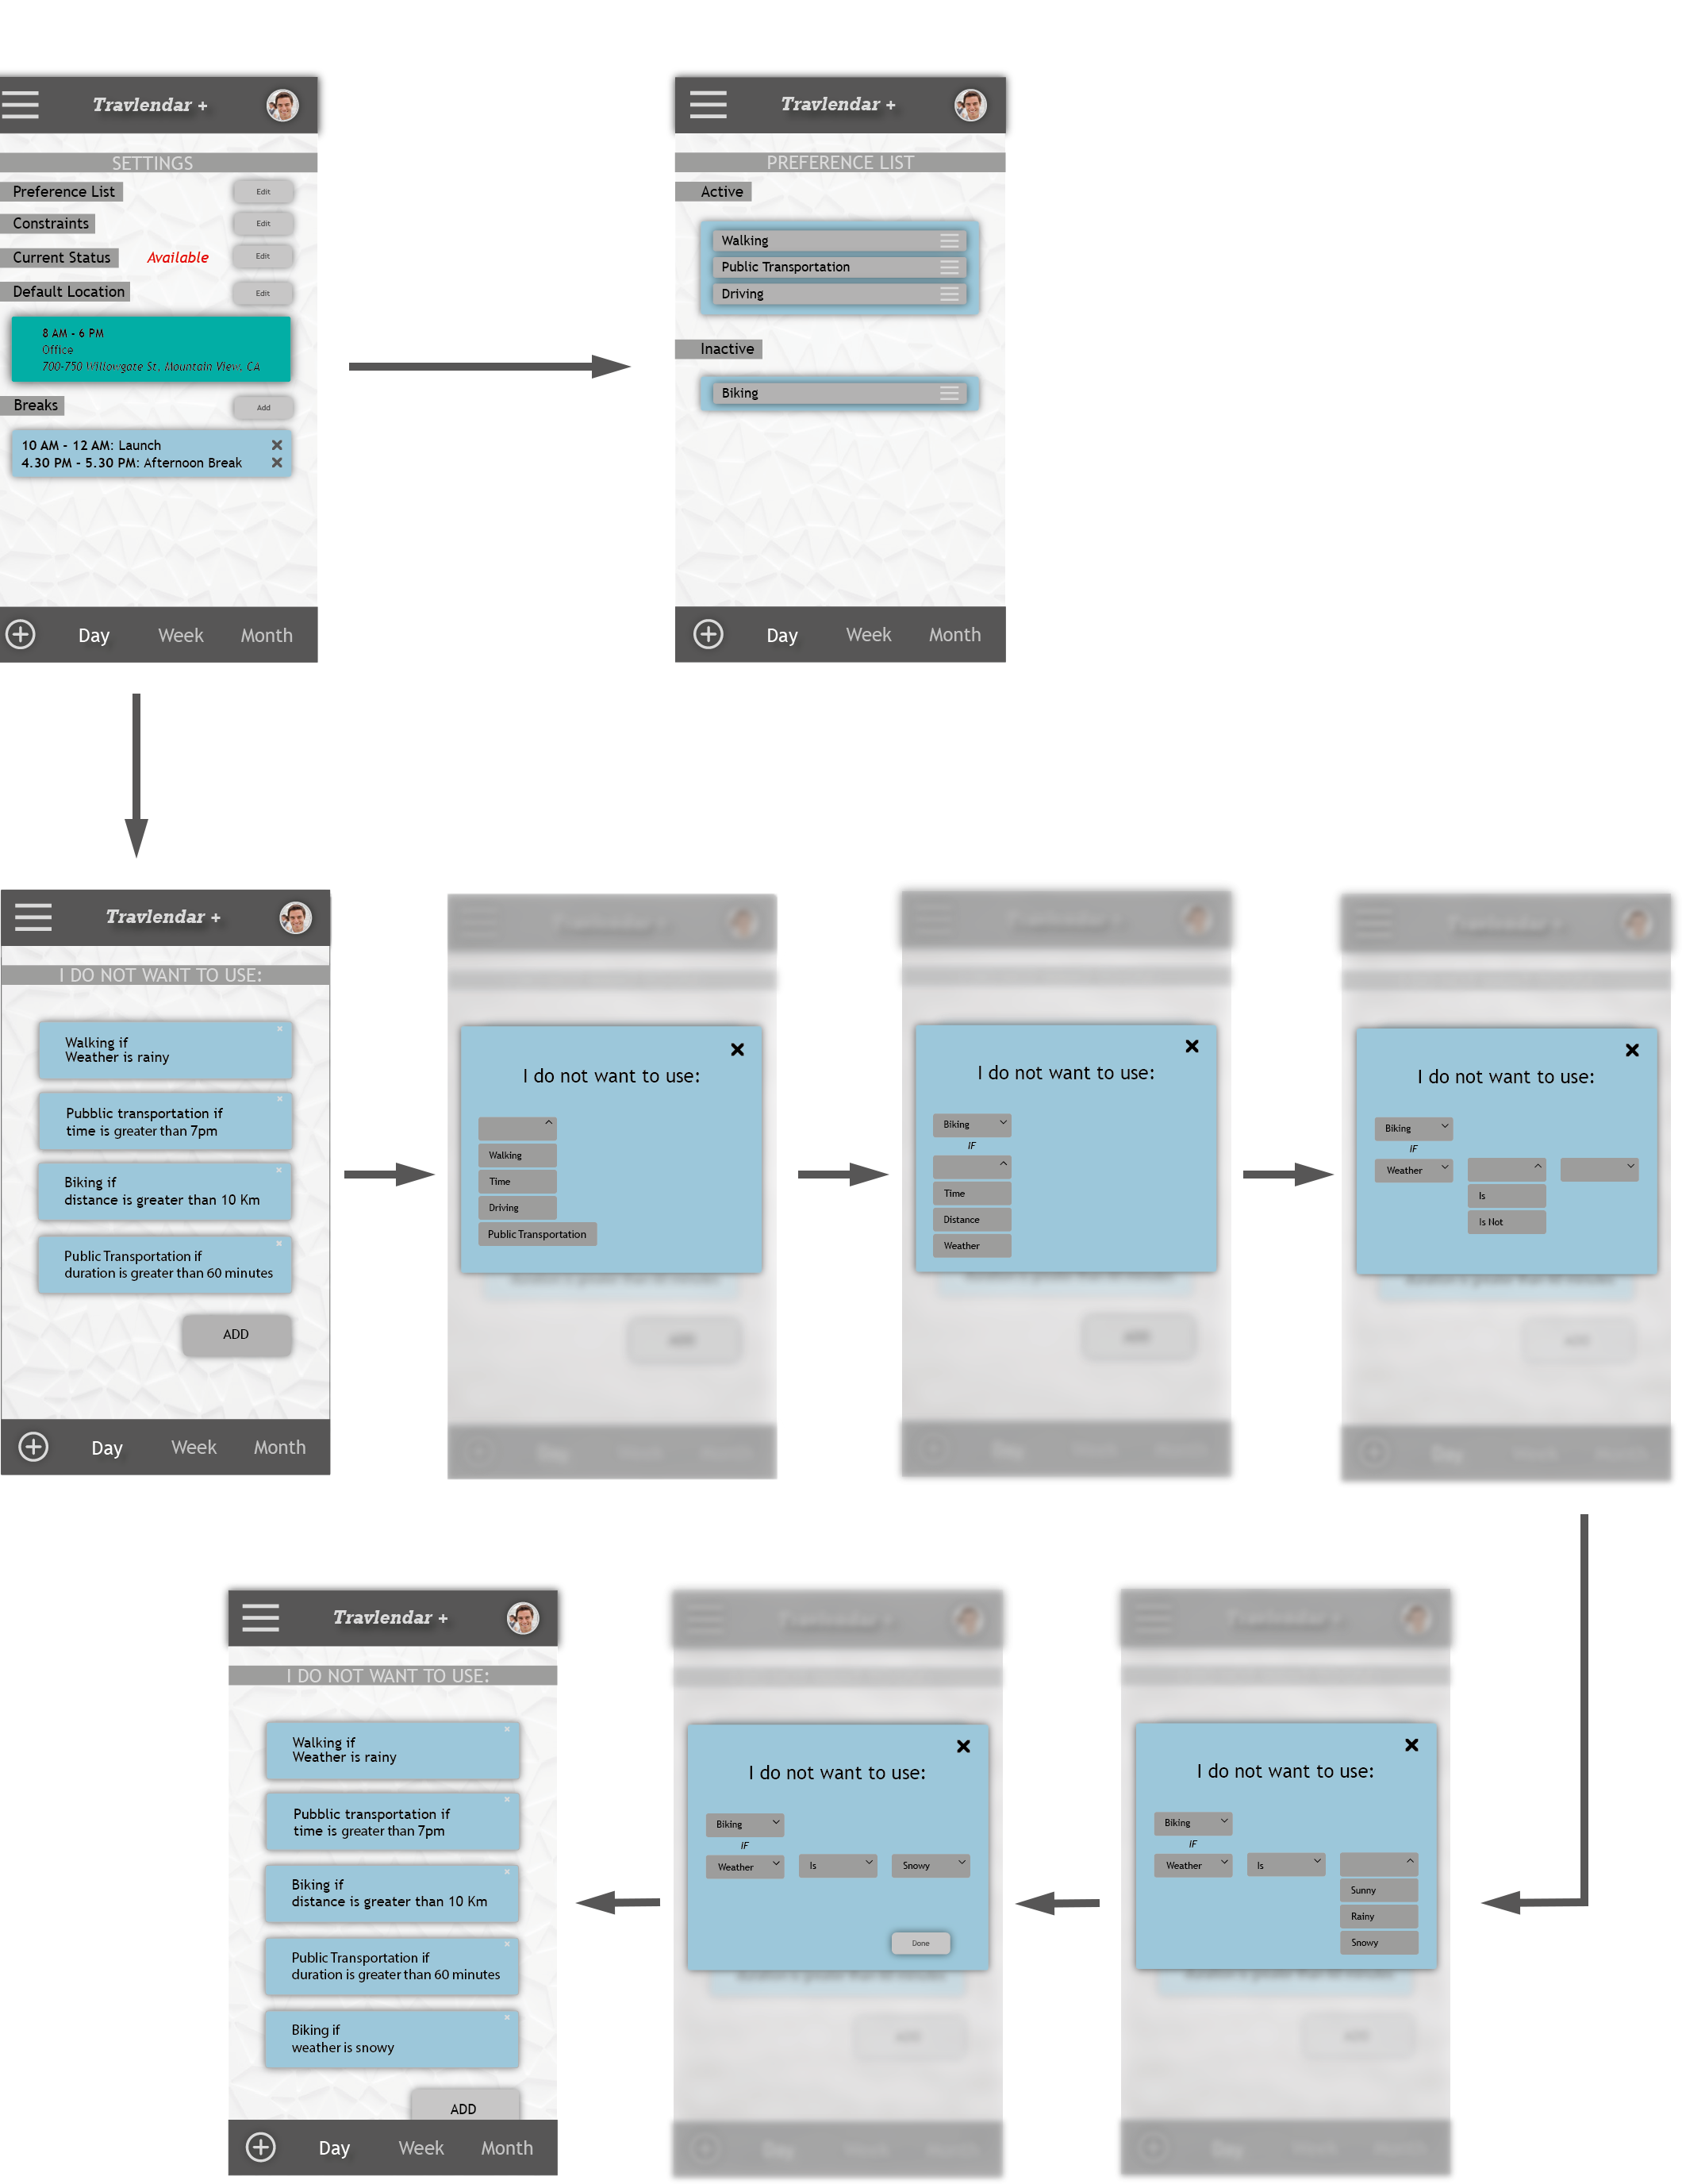
\includegraphics[width = \textwidth, scale = 0.3]{Images/Mockups/Settings+.png}{}
\caption{Settings Mockup}
\end{figure}
\clearpage